\section{Условие}

\subsection{Задание 1}

Назначить адреса подсетей:

\begin{enumerate}
    \item Подсеть 1: 192.168.x.0 /24
    \item Подсеть 2: 192.168.x+1.0 /24
    \item Подсеть 3: 192.168.x+2.0 /24
    \item Подсеть 4: 192.168.x+3.0 /24
    \item Подсеть 5 (В задаче III): 192.168.x+10.0 /24
\end{enumerate}

\subsection{Задание 2}

Настроить динамическую маршрутизацию в прилагаемом .pkt файле на стенде I через протокол RIPv2 так, чтобы пинг любым хостом или маршрутизатором любого другого хоста или маршрутизатора был успешным.

Представить отдельным .pkt файлом. 

\subsection{Задание 3}

Настроить динамическую маршрутизацию в сети в прилагаемом .pkt файле на стенде II через протокол OSPF так, чтобы пинг любым хостом или маршрутизатором любого другого хоста или маршрутизатора был успешным. Разделить при этом сеть на области OSPF в соответствии со схемой. Выполнить указания в лабораторной работе.

Представить отдельным .pkt файлом.

\section{Задание 1}

Стенды были разделены на подсети, указанные в pkt файле. Изображения первого стенда представлено на рисунке \ref{fig:stand1}, а второго -- на \ref{fig:stand2}.

\begin{figure}[H]
    \centering
    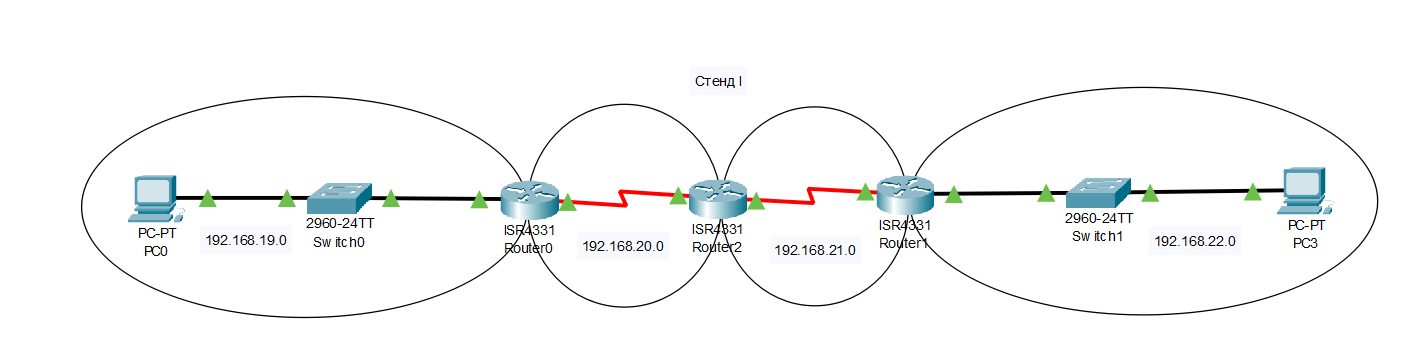
\includegraphics[width=0.8\textwidth]{img/content/stand_1.png}
    \caption{Разделение на подсети на первом стенде}
    \label{fig:stand1}
\end{figure}

\begin{figure}[H]
    \centering
    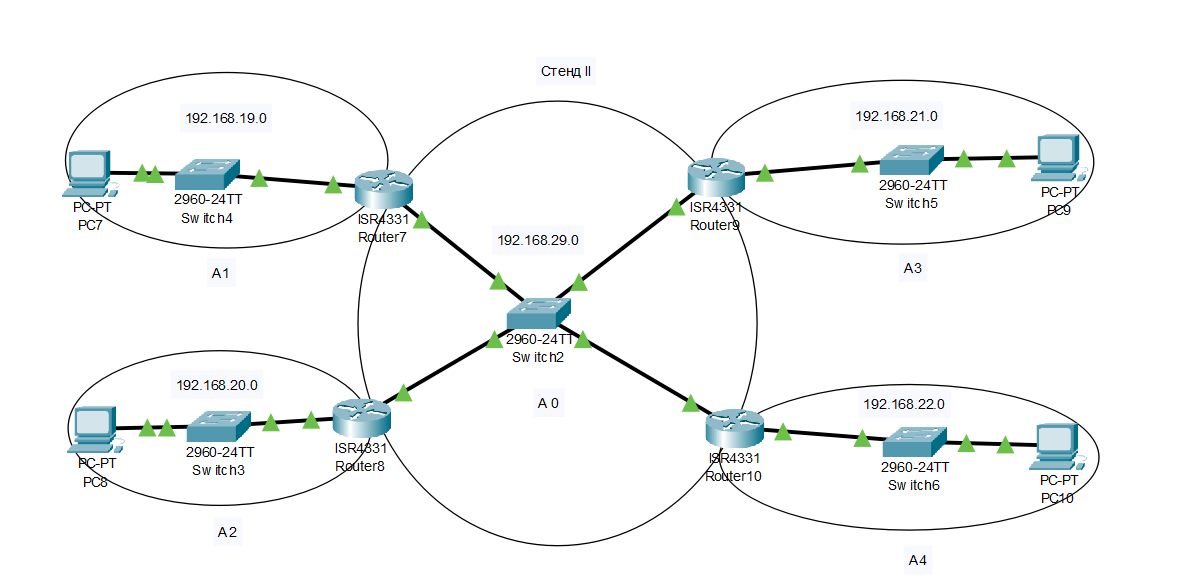
\includegraphics[width=0.8\textwidth]{img/content/stand_2.png}
    \caption{Разделение на подсети на втором стенде}
    \label{fig:stand2}
\end{figure}

\section{Задание 2}

Команды для настройки RIP на Router0 преведены на рисунке \ref{fig:rip}. Для остальных роутеров команды аналогичны.

\begin{figure}[H]
    \centering
    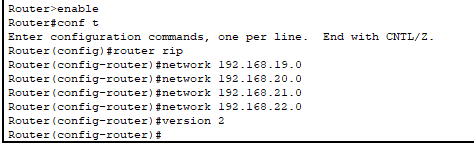
\includegraphics[width=0.8\textwidth]{img/content/rip_router.png}
    \caption{Настройка RIP для Router0 с первого стенда}
    \label{fig:rip}
\end{figure}

На рисунке \ref{fig:ping_1} виден результат проверки соединения между PC0 и PC3 с помощью команды ping.

\begin{figure}[H]
    \centering
    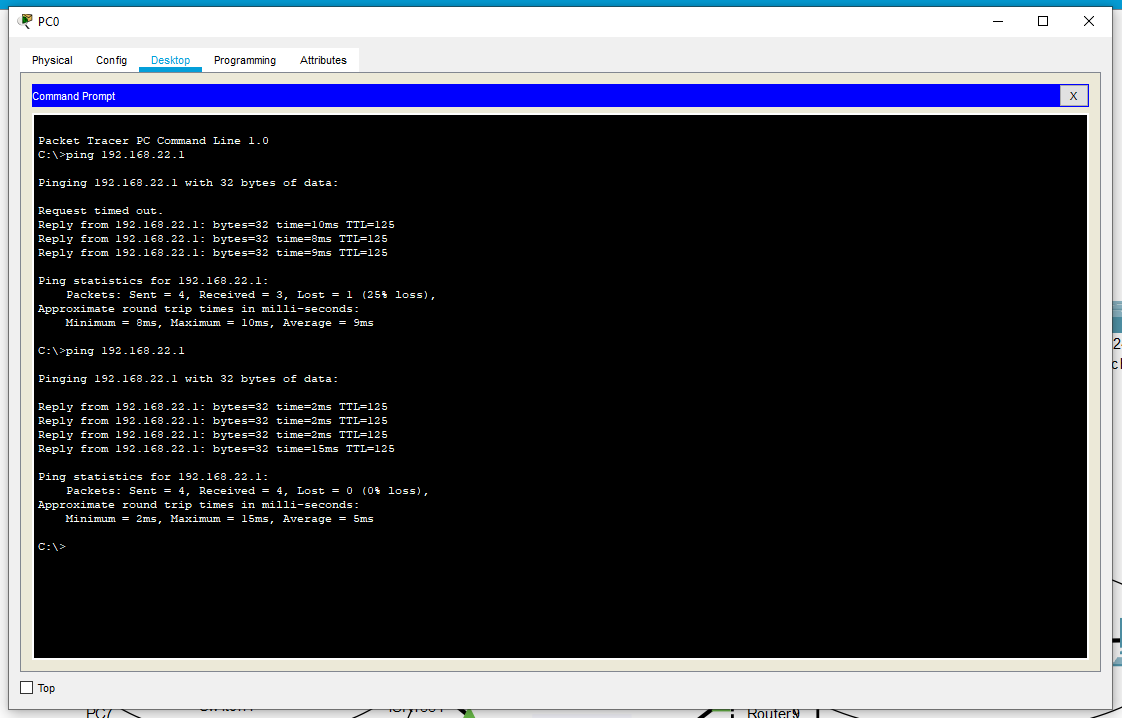
\includegraphics[width=0.8\textwidth]{img/content/ping_1.png}
    \caption{Проверка соединения между PC0 и PC3 с первого стенда}
    \label{fig:ping_1}
\end{figure}

\section{Задача 3}

Для работы протокола OSPF были настроены все роутеры. На рисунках \ref{fig:router7}, \ref{fig:router8}, \ref{fig:router9}, \ref{fig:router10} представлены команды для настройки каждого роутера.

\begin{figure}[H]
    \centering
    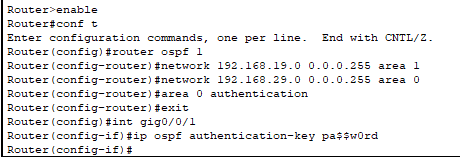
\includegraphics[width=0.8\textwidth]{img/content/router7.png}
    \caption{Настройка OSPF для Router7}
    \label{fig:router7}
\end{figure}

\begin{figure}[H]
    \centering
    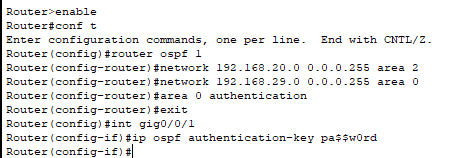
\includegraphics[width=0.8\textwidth]{img/content/router8.png}
    \caption{Настройка OSPF для Router8}
    \label{fig:router8}
\end{figure}

\begin{figure}[H]
    \centering
    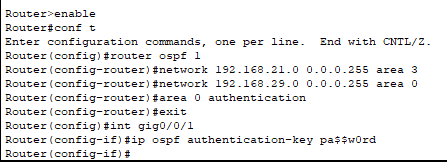
\includegraphics[width=0.8\textwidth]{img/content/router9.png}
    \caption{Настройка OSPF для Router9}
    \label{fig:router9}
\end{figure}

\begin{figure}[H]
    \centering
    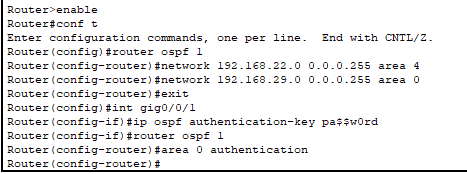
\includegraphics[width=0.8\textwidth]{img/content/router10.png}
    \caption{Настройка OSPF для Router10}
    \label{fig:router10}
\end{figure}

Просмотрим статус соседних устройсв, результат проверки для Router8 изображен на рисунке \ref{fig:neighbor}.

\begin{figure}[H]
    \centering
    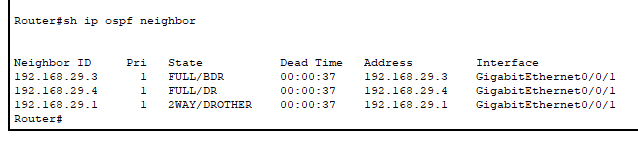
\includegraphics[width=0.8\textwidth]{img/content/router8_neighbor.png}
    \caption{Информация о соседних устройствах для Router8}
    \label{fig:neighbor}
\end{figure}

На рисунке \ref{fig:neighbor} вижно, что роль DR получил Router10, BDR -- Router9. Роль ABR имеют все роутеры, так как каждый из них соединен с разлиными зонами.

На рисунке \ref{fig:ping_1} можно заметить результат проверки соединения между PC7 и PC10.

\begin{figure}[H]
    \centering
    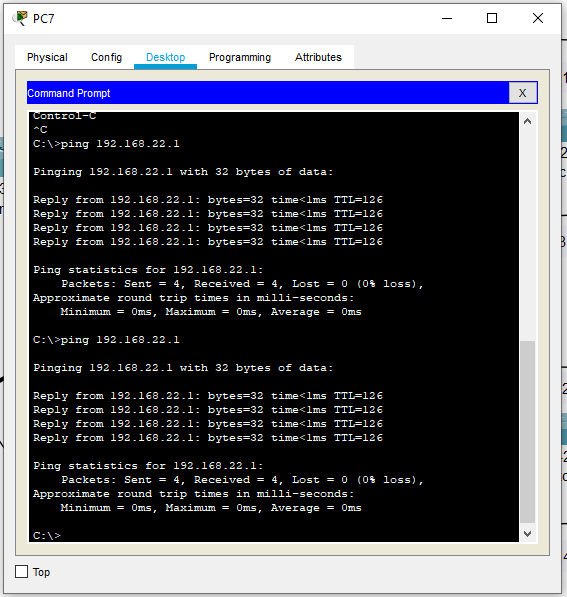
\includegraphics[width=0.8\textwidth]{img/content/ping_2.png}
    \caption{Результат проверки соединения между PC7 и PC10}
    \label{fig:ping_2}
\end{figure}
